
%% bare_conf.tex
%% V1.3
%% 2007/01/11
%% by Michael Shell
%% See:
%% http://www.michaelshell.org/
%% for current contact information.
%%
%% This is a skeleton file demonstrating the use of IEEEtran.cls
%% (requires IEEEtran.cls version 1.7 or later) with an IEEE conference paper.
%%
%% Support sites:
%% http://www.michaelshell.org/tex/ieeetran/
%% http://www.ctan.org/tex-archive/macros/latex/contrib/IEEEtran/
%% and
%% http://www.ieee.org/

%%*************************************************************************
%% Legal Notice:
%% This code is offered as-is without any warranty either expressed or
%% implied; without even the implied warranty of MERCHANTABILITY or
%% FITNESS FOR A PARTICULAR PURPOSE! 
%% User assumes all risk.
%% In no event shall IEEE or any contributor to this code be liable for
%% any damages or losses, including, but not limited to, incidental,
%% consequential, or any other damages, resulting from the use or misuse
%% of any information contained here.
%%
%% All comments are the opinions of their respective authors and are not
%% necessarily endorsed by the IEEE.
%%
%% This work is distributed under the LaTeX Project Public License (LPPL)
%% ( http://www.latex-project.org/ ) version 1.3, and may be freely used,
%% distributed and modified. A copy of the LPPL, version 1.3, is included
%% in the base LaTeX documentation of all distributions of LaTeX released
%% 2003/12/01 or later.
%% Retain all contribution notices and credits.
%% ** Modified files should be clearly indicated as such, including  **
%% ** renaming them and changing author support contact information. **
%%
%% File list of work: IEEEtran.cls, IEEEtran_HOWTO.pdf, bare_adv.tex,
%%                    bare_conf.tex, bare_jrnl.tex, bare_jrnl_compsoc.tex
%%*************************************************************************

% *** Authors should verify (and, if needed, correct) their LaTeX system  ***
% *** with the testflow diagnostic prior to trusting their LaTeX platform ***
% *** with production work. IEEE's font choices can trigger bugs that do  ***
% *** not appear when using other class files.                            ***
% The testflow support page is at:
% http://www.michaelshell.org/tex/testflow/



% Note that the a4paper option is mainly intended so that authors in
% countries using A4 can easily print to A4 and see how their papers will
% look in print - the typesetting of the document will not typically be
% affected with changes in paper size (but the bottom and side margins will).
% Use the testflow package mentioned above to verify correct handling of
% both paper sizes by the user's LaTeX system.
%
% Also note that the "draftcls" or "draftclsnofoot", not "draft", option
% should be used if it is desired that the figures are to be displayed in
% draft mode.
%
\documentclass[conference]{IEEEtran}
\usepackage{blindtext, graphicx}
\usepackage{vntex}
\usepackage{wrapfig}
\usepackage{tabularx}
\usepackage{amsmath}
\usepackage{amssymb}
\newcommand\tab[1][1cm]{\hspace*{#1}}
\usepackage{listings}
\lstset{
basicstyle=\small\ttfamily,
columns=flexible,
breaklines=true
}
\usepackage{caption}
\renewcommand{\thetable}{\arabic{table}}
% Add the compsoc option for Computer Society conferences.
%
% If IEEEtran.cls has not been installed into the LaTeX system files,
% manually specify the path to it like:
% \documentclass[conference]{../sty/IEEEtran}





% Some very useful LaTeX packages include:
% (uncomment the ones you want to load)


% *** MISC UTILITY PACKAGES ***
%
%\usepackage{ifpdf}
% Heiko Oberdiek's ifpdf.sty is very useful if you need conditional
% compilation based on whether the output is pdf or dvi.
% usage:
% \ifpdf
%   % pdf code
% \else
%   % dvi code
% \fi
% The latest version of ifpdf.sty can be obtained from:
% http://www.ctan.org/tex-archive/macros/latex/contrib/oberdiek/
% Also, note that IEEEtran.cls V1.7 and later provides a builtin
% \ifCLASSINFOpdf conditional that works the same way.
% When switching from latex to pdflatex and vice-versa, the compiler may
% have to be run twice to clear warning/error messages.






% *** CITATION PACKAGES ***
%
%\usepackage{cite}
% cite.sty was written by Donald Arseneau
% V1.6 and later of IEEEtran pre-defines the format of the cite.sty package
% \cite{} output to follow that of IEEE. Loading the cite package will
% result in citation numbers being automatically sorted and properly
% "compressed/ranged". e.g., [1], [9], [2], [7], [5], [6] without using
% cite.sty will become [1], [2], [5]--[7], [9] using cite.sty. cite.sty's
% \cite will automatically add leading space, if needed. Use cite.sty's
% noadjust option (cite.sty V3.8 and later) if you want to turn this off.
% cite.sty is already installed on most LaTeX systems. Be sure and use
% version 4.0 (2003-05-27) and later if using hyperref.sty. cite.sty does
% not currently provide for hyperlinked citations.
% The latest version can be obtained at:
% http://www.ctan.org/tex-archive/macros/latex/contrib/cite/
% The documentation is contained in the cite.sty file itself.






% *** GRAPHICS RELATED PACKAGES ***
%
\ifCLASSINFOpdf
  % \usepackage[pdftex]{graphicx}
  % declare the path(s) where your graphic files are
  % \graphicspath{{../pdf/}{../jpeg/}}
  % and their extensions so you won't have to specify these with
  % every instance of \includegraphics
  % \DeclareGraphicsExtensions{.pdf,.jpeg,.png}
\else
  % or other class option (dvipsone, dvipdf, if not using dvips). graphicx
  % will default to the driver specified in the system graphics.cfg if no
  % driver is specified.
  % \usepackage[dvips]{graphicx}
  % declare the path(s) where your graphic files are
  % \graphicspath{{../eps/}}
  % and their extensions so you won't have to specify these with
  % every instance of \includegraphics
  % \DeclareGraphicsExtensions{.eps}
\fi
% graphicx was written by David Carlisle and Sebastian Rahtz. It is
% required if you want graphics, photos, etc. graphicx.sty is already
% installed on most LaTeX systems. The latest version and documentation can
% be obtained at: 
% http://www.ctan.org/tex-archive/macros/latex/required/graphics/
% Another good source of documentation is "Using Imported Graphics in
% LaTeX2e" by Keith Reckdahl which can be found as epslatex.ps or
% epslatex.pdf at: http://www.ctan.org/tex-archive/info/
%
% latex, and pdflatex in dvi mode, support graphics in encapsulated
% postscript (.eps) format. pdflatex in pdf mode supports graphics
% in .pdf, .jpeg, .png and .mps (metapost) formats. Users should ensure
% that all non-photo figures use a vector format (.eps, .pdf, .mps) and
% not a bitmapped formats (.jpeg, .png). IEEE frowns on bitmapped formats
% which can result in "jaggedy"/blurry rendering of lines and letters as
% well as large increases in file sizes.
%
% You can find documentation about the pdfTeX application at:
% http://www.tug.org/applications/pdftex





% *** MATH PACKAGES ***
%
%\usepackage[cmex10]{amsmath}
% A popular package from the American Mathematical Society that provides
% many useful and powerful commands for dealing with mathematics. If using
% it, be sure to load this package with the cmex10 option to ensure that
% only type 1 fonts will utilized at all point sizes. Without this option,
% it is possible that some math symbols, particularly those within
% footnotes, will be rendered in bitmap form which will result in a
% document that can not be IEEE Xplore compliant!
%
% Also, note that the amsmath package sets \interdisplaylinepenalty to 10000
% thus preventing page breaks from occurring within multiline equations. Use:
%\interdisplaylinepenalty=2500
% after loading amsmath to restore such page breaks as IEEEtran.cls normally
% does. amsmath.sty is already installed on most LaTeX systems. The latest
% version and documentation can be obtained at:
% http://www.ctan.org/tex-archive/macros/latex/required/amslatex/math/





% *** SPECIALIZED LIST PACKAGES ***
%
%\usepackage{algorithmic}
% algorithmic.sty was written by Peter Williams and Rogerio Brito.
% This package provides an algorithmic environment fo describing algorithms.
% You can use the algorithmic environment in-text or within a figure
% environment to provide for a floating algorithm. Do NOT use the algorithm
% floating environment provided by algorithm.sty (by the same authors) or
% algorithm2e.sty (by Christophe Fiorio) as IEEE does not use dedicated
% algorithm float types and packages that provide these will not provide
% correct IEEE style captions. The latest version and documentation of
% algorithmic.sty can be obtained at:
% http://www.ctan.org/tex-archive/macros/latex/contrib/algorithms/
% There is also a support site at:
% http://algorithms.berlios.de/index.html
% Also of interest may be the (relatively newer and more customizable)
% algorithmicx.sty package by Szasz Janos:
% http://www.ctan.org/tex-archive/macros/latex/contrib/algorithmicx/




% *** ALIGNMENT PACKAGES ***
%
%\usepackage{array}
% Frank Mittelbach's and David Carlisle's array.sty patches and improves
% the standard LaTeX2e array and tabular environments to provide better
% appearance and additional user controls. As the default LaTeX2e table
% generation code is lacking to the point of almost being broken with
% respect to the quality of the end results, all users are strongly
% advised to use an enhanced (at the very least that provided by array.sty)
% set of table tools. array.sty is already installed on most systems. The
% latest version and documentation can be obtained at:
% http://www.ctan.org/tex-archive/macros/latex/required/tools/


%\usepackage{mdwmath}
%\usepackage{mdwtab}
% Also highly recommended is Mark Wooding's extremely powerful MDW tools,
% especially mdwmath.sty and mdwtab.sty which are used to format equations
% and tables, respectively. The MDWtools set is already installed on most
% LaTeX systems. The lastest version and documentation is available at:
% http://www.ctan.org/tex-archive/macros/latex/contrib/mdwtools/


% IEEEtran contains the IEEEeqnarray family of commands that can be used to
% generate multiline equations as well as matrices, tables, etc., of high
% quality.


%\usepackage{eqparbox}
% Also of notable interest is Scott Pakin's eqparbox package for creating
% (automatically sized) equal width boxes - aka "natural width parboxes".
% Available at:
% http://www.ctan.org/tex-archive/macros/latex/contrib/eqparbox/





% *** SUBFIGURE PACKAGES ***
%\usepackage[tight,footnotesize]{subfigure}
% subfigure.sty was written by Steven Douglas Cochran. This package makes it
% easy to put subfigures in your figures. e.g., "Figure 1a and 1b". For IEEE
% work, it is a good idea to load it with the tight package option to reduce
% the amount of white space around the subfigures. subfigure.sty is already
% installed on most LaTeX systems. The latest version and documentation can
% be obtained at:
% http://www.ctan.org/tex-archive/obsolete/macros/latex/contrib/subfigure/
% subfigure.sty has been superceeded by subfig.sty.



%\usepackage[caption=false]{caption}
%\usepackage[font=footnotesize]{subfig}
% subfig.sty, also written by Steven Douglas Cochran, is the modern
% replacement for subfigure.sty. However, subfig.sty requires and
% automatically loads Axel Sommerfeldt's caption.sty which will override
% IEEEtran.cls handling of captions and this will result in nonIEEE style
% figure/table captions. To prevent this problem, be sure and preload
% caption.sty with its "caption=false" package option. This is will preserve
% IEEEtran.cls handing of captions. Version 1.3 (2005/06/28) and later 
% (recommended due to many improvements over 1.2) of subfig.sty supports
% the caption=false option directly:
%\usepackage[caption=false,font=footnotesize]{subfig}
%
% The latest version and documentation can be obtained at:
% http://www.ctan.org/tex-archive/macros/latex/contrib/subfig/
% The latest version and documentation of caption.sty can be obtained at:
% http://www.ctan.org/tex-archive/macros/latex/contrib/caption/




% *** FLOAT PACKAGES ***
%
%\usepackage{fixltx2e}
% fixltx2e, the successor to the earlier fix2col.sty, was written by
% Frank Mittelbach and David Carlisle. This package corrects a few problems
% in the LaTeX2e kernel, the most notable of which is that in current
% LaTeX2e releases, the ordering of single and double column floats is not
% guaranteed to be preserved. Thus, an unpatched LaTeX2e can allow a
% single column figure to be placed prior to an earlier double column
% figure. The latest version and documentation can be found at:
% http://www.ctan.org/tex-archive/macros/latex/base/



%\usepackage{stfloats}
% stfloats.sty was written by Sigitas Tolusis. This package gives LaTeX2e
% the ability to do double column floats at the bottom of the page as well
% as the top. (e.g., "\begin{figure*}[!b]" is not normally possible in
% LaTeX2e). It also provides a command:
%\fnbelowfloat
% to enable the placement of footnotes below bottom floats (the standard
% LaTeX2e kernel puts them above bottom floats). This is an invasive package
% which rewrites many portions of the LaTeX2e float routines. It may not work
% with other packages that modify the LaTeX2e float routines. The latest
% version and documentation can be obtained at:
% http://www.ctan.org/tex-archive/macros/latex/contrib/sttools/
% Documentation is contained in the stfloats.sty comments as well as in the
% presfull.pdf file. Do not use the stfloats baselinefloat ability as IEEE
% does not allow \baselineskip to stretch. Authors submitting work to the
% IEEE should note that IEEE rarely uses double column equations and
% that authors should try to avoid such use. Do not be tempted to use the
% cuted.sty or midfloat.sty packages (also by Sigitas Tolusis) as IEEE does
% not format its papers in such ways.





% *** PDF, URL AND HYPERLINK PACKAGES ***
%
%\usepackage{url}
% url.sty was written by Donald Arseneau. It provides better support for
% handling and breaking URLs. url.sty is already installed on most LaTeX
% systems. The latest version can be obtained at:
% http://www.ctan.org/tex-archive/macros/latex/contrib/misc/
% Read the url.sty source comments for usage information. Basically,
% \url{my_url_here}.





% *** Do not adjust lengths that control margins, column widths, etc. ***
% *** Do not use packages that alter fonts (such as pslatex).         ***
% There should be no need to do such things with IEEEtran.cls V1.6 and later.
% (Unless specifically asked to do so by the journal or conference you plan
% to submit to, of course. )


% correct bad hyphenation here
\hyphenation{op-tical net-works semi-conduc-tor}


\begin{document}
\pagenumbering{arabic}
%
% paper title
% can use linebreaks \\ within to get better formatting as desired
\title{
  Bài dự thi Olympic Kinh tế lượng (Bản tóm tắt)\\
  Xây dựng công cụ hỗ trợ dự đoán giá trị Bitcoin bằng Học máy
}

% author names and affiliations
% use a multiple column layout for up to three different
% affiliations
\author{
  \IEEEauthorblockN{Phan Sơn Tự}
  \IEEEauthorblockA{
    Đại học Bách Khoa TP. Hồ Chí Minh\\
    Khoa Khoa học và Kĩ thuật Máy tính\\
    Email: phan.son.tu.1994@gmail.com - SĐT: 0164.9766.574
  }
}

% conference papers do not typically use \thanks and this command
% is locked out in conference mode. If really needed, such as for
% the acknowledgment of grants, issue a \IEEEoverridecommandlockouts
% after \documentclass

% for over three affiliations, or if they all won't fit within the width
% of the page, use this alternative format:
% 
%\author{\IEEEauthorblockN{Michael Shell\IEEEauthorrefmark{1},
%Homer Simpson\IEEEauthorrefmark{2},
%James Kirk\IEEEauthorrefmark{3}, 
%Montgomery Scott\IEEEauthorrefmark{3} and
%Eldon Tyrell\IEEEauthorrefmark{4}}
%\IEEEauthorblockA{\IEEEauthorrefmark{1}School of Electrical and Computer Engineering\\
%Georgia Institute of Technology,
%Atlanta, Georgia 30332--0250\\ Email: see http://www.michaelshell.org/contact.html}
%\IEEEauthorblockA{\IEEEauthorrefmark{2}Twentieth Century Fox, Springfield, USA\\
%Email: homer@thesimpsons.com}
%\IEEEauthorblockA{\IEEEauthorrefmark{3}Starfleet Academy, San Francisco, California 96678-2391\\
%Telephone: (800) 555--1212, Fax: (888) 555--1212}
%\IEEEauthorblockA{\IEEEauthorrefmark{4}Tyrell Inc., 123 Replicant Street, Los Angeles, California 90210--4321}}




% use for special paper notices
%\IEEEspecialpapernotice{(Invited Paper)}




% make the title area
\maketitle
\thispagestyle{plain}
\pagestyle{plain}


\begin{abstract}
% \boldmath
Vấn đề cơ bản của việc đầu tư là lợi nhuận, bám sát với mục tiêu này phương hướng 
đề ra sẽ đi giải quyết bài toán cụ thể như sau:\\
Sử dụng USD (US Dollar) để mua/bán BTC (Bitcoin), với mỗi phiên giao dịch là 30 phút, chúng 
ta sẽ đi dự đoán giá trị BTC trong phiên tiếp theo sẽ tăng hay giảm - bài
toán phân lớp trong Học máy. Để thực hiện được điều đó bài dự thi vạch ra những bước đi cụ
thể để hiện thực mục tiêu: (1) Thu thập, xử lí dữ liệu BTC; (2) Áp dụng các giải 
thuật phân lớp vào tập dữ liệu có được; (3) Đánh giá trên lý thuyết hệ thống; (3) 
Vận hành, khảo sát và đánh giá hệ thống trên thực tế; (4) Xây dựng, hoàn thiện sản 
phẩm.\\
Sản phẩm hoàn thiện mà người dùng được sử dụng sẽ là một ứng dụng nền web cung 
cấp các thông tin về dự đoán và các thông số thống kê dùng để tham khảo cho việc 
đầu tư.
\end{abstract}
% IEEEtran.cls defaults to using nonbold math in the Abstract.
% This preserves the distinction between vectors and scalars. However,
% if the journal you are submitting to favors bold math in the abstract,
% then you can use LaTeX's standard command \boldmath at the very start
% of the abstract to achieve this. Many IEEE journals frown on math
% in the abstract anyway.

% Note that keywords are not normally used for peerreview papers.
% \begin{IEEEkeywords}
% IEEEtran, journal, \LaTeX, paper, template.
% \end{IEEEkeywords}






% For peer review papers, you can put extra information on the cover
% page as needed:
% \ifCLASSOPTIONpeerreview
% \begin{center} \bfseries EDICS Category: 3-BBND \end{center}
% \fi
%
% For peerreview papers, this IEEEtran command inserts a page break and
% creates the second title. It will be ignored for other modes.
\IEEEpeerreviewmaketitle


\section{Giới thiệu đề tài}
Bitcoin - một hệ thống tiền mã hóa (hay tiền điện tử) được xuất hiện lần đầu tiên 
vào năm 2009 bởi Satoshi Nakamoto \cite{BitcoinPaper}, với những đặc tính ưu việt hơn cả tiền tệ 
truyền thống hiện nay đã khiến cho sự tăng lên nhanh chóng về giá trị. Nhận thấy 
được sức mạnh của tiền mã hóa có thể sẽ là tương lai của kinh tế và chính trị 
nên việc hiểu rõ cũng như đầu tư vào Bitcoin là việc đáng để quan tâm.\\\\
Trong giai đoạn hiện nay, đối với nước ta, Bitcoin là một khái niệm mới vì thế 
mà việc đầu tư khi chưa có nền tảng kiến thức hoặc kinh nghiệm đầu tư là hết 
sức rủi ro. Nhận thấy vấn đề này, bản thân xây dựng một công cụ để cho nhà đầu 
tư có thể dựa vào như một yếu tố tham khảo tin cậy.\\\\
Trên một sàn giao dịch tiền mã hóa điển hình, quá trình mua bán BTC được chia ra 
thành các giai đoạn thời gian và được gọi là phiên giao dịch. Một phiên giao dịch 
được diễn tả bởi các giá trị điển hình như sau:
\begin{itemize}
\item Giá mở phiên: giá bán (mua) BTC của (các) giao dịch ngay tại thời 
điểm mở phiên.
\item Giá đóng phiên: giá bán (mua) BTC của (các) giao dịch tại thời điểm 
kết thúc phiên.
\item Giá cao nhất: giá bán (mua) BTC cao nhất của giao dịch trong khoảng 
thời gian mở phiên đến kết thúc phiên.
\item Giá thấp nhất: giá bán (mua) BTC thấp nhất của giao dịch trong khoảng 
thời gian mở phiên đến kết thúc phiên.
\end{itemize}
Thời gian của một phiên giao dịch thường được chọn là 5 phút, 30 phút, 1 tiếng, 2 tiếng, 
4 tiếng hoặc 1 ngày, ... 
Trong phạm vi đề tài chúng ta chọn thời gian một phiên giao dịch là 30 phút.\\\\
Vậy, bài toán cần giải quyết là đi dự đoán giá trị BTC trong phiên tiếp theo sẽ tăng 
hay giảm so với phiên hiện tại. Cụ thể, gọi $n$ là phiên hiện tại và $n_{close}$ 
là giá đóng phiên hiện tại, $(n+1)$ là phiên tiếp theo và $(n+1)_{close}$ là giá đóng 
phiên tiếp theo. Nếu $(n+1)_{close} > n_{close}$ thì giá tăng - $Up$, ngược lại thì, 
$(n+1)_{close} \leq n_{close}$ thì giá giảm - $Down$.\\\\
Sau khi cụ thể được yêu cầu bài toán, ta sẽ đi đặc tả hướng tiếp cận giải quyết 
vấn đề. Học máy là lựa chọn của đề tài này, cụ thể phương pháp giải quyết 
sẽ sử dụng giải thuật phân lớp để dự đoán nhãn của phiên giao dịch sẽ là $Up$ 
hay $Down$. 
\section{Nền tảng lý thuyết}

\subsection{Sơ lược về Bitcoin}
Các hình thức thương mại trên Internet ngày nay hầu như đều dựa vào một tổ chức 
bên thứ ba đáng tin cậy để xử lý các hoạt động thanh toán điện tử. Tuy rằng sau 
nhiều năm phát triển, các tổ chức bên thứ ba này đều đã nâng cao mức độ tin cậy, 
an toàn nhưng đa số vẫn còn tồn tại những điểm yếu: không thể tránh khỏi những 
tranh chấp, phí trung gian, đòi hòi phải cung cấp các thông tin cá nhân... Và 
Bitcoin - hệ thống tiền điện tử ngang hàng (A Peer-to-Peer Electronic Cash System) 
được sinh ra để giải quyết các vấn đề trên \cite{BitcoinPaper}.\\\\
Khi so sánh với tiền tệ truyền thống, Bitcoin có hình thức và cách thức hoạt 
động khác biệt. Bitcoin không hề có bất kỳ một tổ chức tập trung nào để quản 
lý, thay vào đó, Bitcoin sử dụng mạng ngang hàng để hoạt động \cite{Bitcoin1}.
\\\\
Trong cách viết, Bitcoin được hiểu như một hệ thống, giao thức hoặc một cộng 
đồng, cụ thể trong phạm vi bài dự thi này, Bitcoin được hiểu là một hệ thống. Còn 
BTC được hiểu là một tài sản hoặc một đơn vị tiền tệ.\\\\
BTC được sinh ra bằng cách sử dụng các tài nguyên phần cứng và năng lượng (CPU, 
GPU, phần cứng ASIC, điện năng...) để đi giải một ``câu đố mã hóa'', phần thưởng 
cho người chiến thắng chính là BTC. Trong thời gian đầu (210.000 block đầu tiên) 
(tham khảo về block ở mục 3.1.5), phần thưởng là 50 BTC và các giai đoạn sau sẽ giảm 
dần đi một nửa (25 BTC, 12.5 BTC ...) cứ sau khoảng 210.000 block. Đặc biệt, số 
lượng BTC là hữu hạn và chính xác là 21 triệu BTC, ước tính đến năm 2140 lượng 
BTC khai thác sẽ cạn kiệt \cite{Bitcoin2}. Cũng chính tính chất này là một trong 
những yếu tố tạo nên giá trị của BTC, vì bị giới hạn số lượng nên BTC có tính 
khan hiếm và không bị lạm phát, các tính chất này khác biệt so với tiền tệ 
truyền thống và được ví như vàng 2.0 - vàng của mạng Internet.\\\\
Ngoài các yếu tố vượt trội trên, Bitcoin còn được xây dựng là một hệ thống có 
tính chất ẩn danh, các địa chỉ chứa BTC đều là những dãy ký tự trừu tượng, không 
có ý nghĩa về mặt xác minh cá nhân và rất khó để biết ai là chủ nhân thật sự của 
một địa chỉ. Mặc dù, Bitcoin có tính ẩn danh nhưng tất cả những giao dịch trên 
hệ thống đều được công khai, điều đó có nghĩa là một giao dịch phải được sự xác 
minh về tính hợp lệ của đa số các thành viên trong mạng. Việc xác minh dựa vào các 
quan hệ, cấu trúc liên quan đến toán học, mật mã... \cite{Bitcoin1, BitcoinPaper}\\\\
Tính công khai của Bitcoin được thể hiện ở quá trình xác minh các giao dịch, 
ngoài ra nó còn được thể hiện ở phương diện kỹ thuật, các mã nguồn lập trình 
và các đoạn lập trình đều được công bố công khai.\\\\
Đơn vị giao dịch, BTC có thể được chia thành nhiều đơn vị nhỏ hơn, tối thiểu 
là đơn vị $Satoshi$. Cụ thể $1 \, Satoshi = 0.01 \, \mu BTC = 0.00000001 \, BTC$ 
hoặc $1 \, BTC = 100.000.000 \, Satoshi$ \cite{Bitcoin3}.

\subsection{Một số khái niệm về tài chính}
\subsubsection{Giới thiệu về sàn giao dịch}
Sàn giao dịch là một thị trường có tính tổ chức cao, nơi các tài sản giao dịch 
có thể trao đổi bằng vật ngang giá (tiền tệ, hợp đồng, ...). Trong phạm vi đề 
tài này khi nhắc đến sàn giao dịch ta hiểu rằng đây là sàn giao dịch với tài 
sản giao dịch là BTC và vật ngang giá là USD.
\subsubsection{Phiên giao dịch và các giá trị cơ bản}
Gọi $T$ là một mốc thời gian bất kỳ, $P$ là khoảng thời gian được chọn là một 
phiên giao dịch. Ta có thể nói một cách đơn giản là phiên giao dịch được mở tại 
thời điểm $T$ và được kết thúc tại thời điểm $T + P$.\\\\
Cụ thể, giả sử chọn mốc mở phiên là 9:00am và phiên giao dịch có thời hạn là 
30 phút, điều đó có nghĩa là kết thúc phiên giao dịch sẽ là 9:30am.\\\\
Các thông tin của một phiên giao dịch:
\begin{itemize}
\item Giá mở phiên: là giá bán của một giao dịch gần nhất sau thời điểm $T$. Ví 
dụ tại thời điểm 9:01am có một giao dịch bán 1 BTC là \$779 và trong khoảng thời 
gian 9:00am đến 9:01am không hề có bất kỳ giao dịch nào khác ngoại trừ giao dịch 
này, thì ta có thể nói giá mở phiên sẽ là \$779.
\item Giá đóng phiên: là giá bán của một giao dịch gần nhất trước thời điểm 
$T + P$.
\item Giá phiên cao nhất: là giá bán cao nhất của một giao dịch trong khoảng 
thời gian diễn ra phiên giao dịch, cụ thể là từ thời điểm $T$ đến thời điểm 
$T + P$. Ví dụ, trong khoảng thời gian 9:00am (thời điểm mở phiên) đến thời gian 
9:30am (thời điểm đóng phiên) có một giao dịch BTC với giá là \$801 và là giao 
dịch có giá trị cao nhất. Vậy ta có thể nó giá phiên cao nhất là \$801.
\item Giá phiên thấp nhất: là giá bán thấp nhất của một giao dịch trong khoảng 
thời gian diễn ra phiên giao dịch, cụ thể là từ thời điểm $T$ đến thời điểm $T + P$.
\item Lượng giao dịch: tổng giá trị USD được dùng để  mua/bán BTC trong một phiên 
giao dịch.
\item Trung bình giao dịch: giá trị USD trung bình của tất cả các giao dịch diễn 
ra trong khoảng thời gian một phiên giao dịch.
\end{itemize}
\subsubsection{Tính thanh khoản}
Tính thanh khoản là đặc trưng chỉ mức độ mà một tài sản bất kì có thể được mua 
hoặc bán trên thị trường mà không làm ảnh hưởng đến giá thị trường của tài sản 
đó. Một tài sản có tính thanh khoản cao nếu có thể được bán nhanh chóng mà giá 
bán giảm không đáng kể. Trong kế toán, tài sản lưu động có thể được chia làm 5 
loại và được sắp xếp theo tính thanh khoản từ cao đến thấp như sau: tiền mặt, 
đầu tư ngắn hạn, khoản phải thu, ứng trước ngắn hạn và hàng tồn kho. Trong đó, 
tiền mặt có tính thanh khoản cao nhất vì luôn luôn dùng được trực tiếp để thanh 
toán, lưu thông, tích trữ.\\\\
Cách gọi thay thế khác cho tính thanh khoản đó là tính lỏng hoặc tính lưu động.
\subsubsection{Quá mua và Quá bán}
Quá mua (Overbought) dùng để định nghĩa trường hợp thị trường có mức cầu cao hơn 
mức cung, điều này làm đẩy giá của tài sản giao dịch lên cao vượt qua mức chính 
đáng. Ví dụ, trên tất cả các giao dịch có hơn 80\% lệnh là đặt mua và dưới 20\% 
là lệnh đặt bán, trường hợp này được xem là quá mua.\\\\
Ngược lại, quá bán (Oversold) dùng để định nghĩa trường hợp thị trường có mức 
cung cao hơn mức cầu, điều này làm kéo giá của tài sản giao dịch xuống thấp vượt 
mức chính đáng.
\subsubsection{Chỉ số dao động ngẫu nhiên}
Chỉ số dao động ngẫu nhiên (Stochastic Oscillator) là đại lượng dùng để đo xu 
hướng mua/bán của thị trường tại thời điểm phiên $x$ thông qua $n$ phiên trước 
đó. Giả sử:\\\\
\tab $L_{n} = $ giá phiên thấp nhất trong $n$ phiên\\
\tab $H_{n} = $ giá phiên cao nhất trong $n$ phiên\\
\tab $P(x) = $ giá của ngày $x$
\[\%K=\frac{P(x)-L_{n}}{H_{n}-L_{n}}\]
Nếu $ \%K $ nhỏ hơn 20 thì thị trường đang có xu hướng quá bán và nếu lớn hơn 
80 thì thị trường đang có xu hướng quá mua.
\subsubsection{Tỉ lệ thay đổi}
Tỉ lệ thay đổi (Rate of Change) là đại lượng đo sự khác nhau của giá tại phiên 
thứ $x$ so với $n$ phiên trước đó. Giá sử $P(x)$ là giá của phiên thứ $x$ thì:
\[ ROC_{n}(x)=\frac{P(x)-P(x-n)}{P(x-n)}\]
Nếu $ROC > 0$ thì giá thị trường đang có xu hướng đi lên (tăng giá).
Ngược lại, với $ROC < 0$ thì giá thị trường đang có xu hướng giảm xuống.

\subsection{Mạng neural (Học máy)}
Học sâu là một nhánh của Học máy, đại diện cho hướng tiếp cận gần với cái nhìn 
thực tế, học nhiều cấp và học từ bản chất dữ liệu. Học sâu thường giải quyết 
rất tốt với các loại dữ liệu mang tính ``con người'' như hình ảnh, âm thanh ... 
\cite{NeuralNetworksandDeepLearning} 
\subsubsection{Cấu trúc một perceptron}
Một perceptron sẽ có các giá trị đầu vào $x_1, x_2, ...$, giá trị đầu ra sẽ 
là kết quả toán học của các giá trị đầu vào và là một giá trị nhị phân.\\
\begin{figure}[h!]
\centering

\includegraphics[height=1in, keepaspectratio=true]{perceptron_n.png}
\caption{Perceptron}
\end{figure}\\
Biểu diễn đại số:
\[
  output = 
  \bigg\{
    _{0 \quad if \, \sum_j w_j x_j \, \leq \, threshold}
    ^{1 \quad if \, \sum_j w_j x_j \, > \, threshold}
\]
Các hàm số như trên được gọi là hàm hoạt động - activation function, có nhiều 
loại hàm hoạt động khác nhau như: $sigmoid , tang ...$
\subsubsection{MNN (Multilayer Neural Network)}
MNN được cấu thành bằng cách sắp xếp các perceptron thành 
từng lớp. Các perceptron ở mỗi lớp sẽ kết nối với tất cả các perceptron ở các 
lớp liền kề, lớp những perceptron đầu tiên được gọi là lớp đầu vào (input layer), 
chúng có chức năng tiếp nhận các giá trị đầu vào để cung cấp cho các lớp tiếp 
theo. Các giá trị đầu ra ở lớp trước sẽ chính là các giá trị đầu vào cho 
các perceptron ở lớp tiếp theo. Các perceptron ở lớp cuối cùng được gọi là lớp 
đầu ra (output layer), trong trường hợp này đặc biệt chỉ có duy nhất một 
perceptron ở lớp đầu ra. Còn lại các lớp perceptron khác được gọi là lớp ẩn 
(hidden layer).\\
\begin{figure}[h!]
\centering
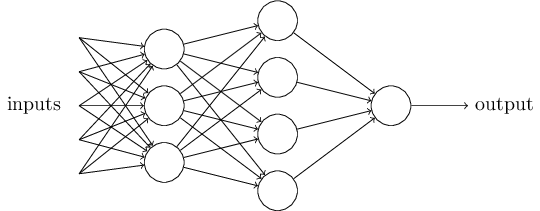
\includegraphics[height=1.25in, keepaspectratio=true]{multilayerneuralnetwork.png}
\caption{MNN}
\end{figure}\\
Giả sử đầu vào của perceptron là $x_1, x_2, ...$ tương ứng là đó là các trọng 
số $w_1, w_2, ...$. Thêm vào định nghĩa về $bias$, ở đây $bias$ là một giá trị 
đại diện độ lệch của từng perceptron và được ký hiệu $b_1, b_2, ...$. Ta có 
biểu diễn của hàm hoạt động với $bias$:
\[
  output = 
  \bigg\{
    _{0 \quad if \, \sum_j w_j x_j + b_i\, \leq \, 0}
    ^{1 \quad if \, \sum_j w_j x_j + b_i\, > \, 0}
\]
\subsubsection{Hàm sigmoid}
Với hàm hoạt động được định nghĩa như trên, giá trị của hàm hoạt động trên lý 
thuyết là không có giới hạn, nghĩa là $output\in\mathbb{R}$. Trong một trường 
hợp cụ thể, với việc sử dụng hàm hoạt động như trên có thể dẫn đến trường hợp 
đầu ra của một perceptron sẽ nhận giá trị rất lớn - giả sử là 1000, những một 
perceptron khác sẽ nhận giá trị rất bé - giả sử 0.001. Vì thế khi đến lớp tiếp 
theo thì gần như perceptron cho kết quả đầu ra là giá trị bé sẽ mất đi độ ảnh 
hưởng và làm mất cân đối cho toàn mạng.\\\\
Do đó để giới hạn giá trị đầu ra của hàm hoạt động chúng ta sẽ sử dụng hàm 
sigmoid. Hàm sigmoid được định nghĩa như sau:
\[
  \sigma(z)=\frac{1}{1+e^{-z}}
\]
Với biễu diễn đồ thị:
\begin{figure}[h!]
\centering
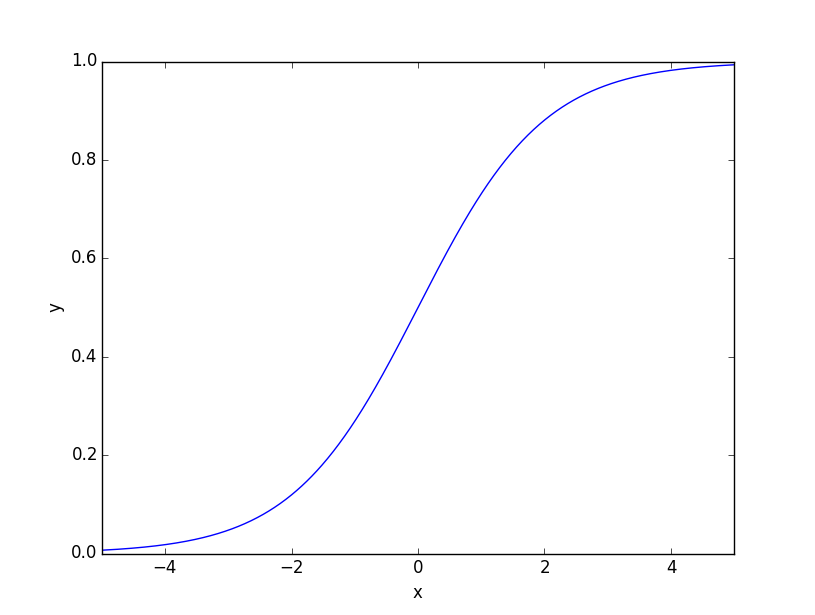
\includegraphics[height=2in, keepaspectratio=true]{sigmoid.png}
\caption{Đồ thị hàm sigmoid}
\end{figure}\\
Áp dụng hàm sigmoid vào hàm hoạt động ta có một hàm hoạt động dạng sigmoid và 
khi đó hàm hoạt động của chúng ta của chúng ta sẽ có dạng:
\[
  \frac{1}{1+exp(-\sum_j w_j x_j -b)}
\]
Lúc này ta có một hàm hoạt động có giá trị được giới hạn trong khoảng từ 0 đến 
1. Nhưng chú ý, giá trị đầu ra của hàm hoạt động vẫn là giá trị liên tục, để 
rời rạc hóa giá trị đầu ra của hàm hoạt động ta có thể sử dụng một phương pháp 
quen thuộc - sử dụng ngưỡng. Điển hình ta chọn ngưỡng $threshold = 0.5$, nếu 
lớn hơn ngưỡng thì giá trị đầu ra của hàm hoạt động sẽ nhận 1 và ngược lại sẽ 
nhận 0.
\subsubsection{Giải thuật lan truyền ngược}
Giải thuật lan truyền ngược cung cấp cho mạng neural khả năng tự học hỏi từ 
đó để bản thân mạng có thể tự xây dựng mô hình 
quyết định và đưa ra các giá trị đầu ra tương ứng với từng trường hợp đầu vào 
cụ thể.\\\\
Cụ thể, MNN với hàm hoạt động có dạng
sigmoid và các tham số $w, b$, các tham số này chưa có giá trị.  Việc cung 
cấp khả năng tự học hỏi cho mạng chính là cung cấp một giải thuật giúp mạng 
tìm được các tham số $w, b$ với một tập kinh nghiệm - hay tập huấn luyện - 
${x, y}$ cụ thể, trong đó $x$ là giá trị đầu vào và $y$ là giá trị đầu ra 
tương ứng với từng bộ $x$. Giải thuật lan truyền ngược là một giải thuật giúp 
giải quyết vấn đề trên.\\\\
Biểu diễn trọng số, $bias$ và hàm hoạt động:\\\\
Trọng số $w_{jk}^\ell$ là trọng số từ lớp perceptron thứ $k$ của lớp $(\ell-1)$ 
đến perceptron thứ j thuộc lớp thứ $\ell$.
Như hình trên, trọng số xuất phát từ perceptron thứ 4 thuộc lớp thứ 2 và kết 
thúc tại perceptron thứ 2 thuộc lớp thứ 3 được ký hiệu là $w_{24}^3$.\\
\begin{figure}[h!]
\centering

\includegraphics[height=2in, keepaspectratio=true]{exw.png}
\caption{Ký hiệu trọng số}
\end{figure}\\
Tương tự như vậy với $bias$ và hàm hoạt động của perceptron thứ $j$ thuộc lớp 
thứ $\ell$ của mạng sẽ được kí hiệu thứ tự là $b_j^\ell,\,a_j^\ell$. Ví dụ, $bias$ 
của perceptron thứ 3 thuộc lớp thứ 2 sẽ là $b_3^2$ và hàm hoạt động của 
perceptron thứ 1 thuộc lớp thứ 3 sẽ là $a_1^3$.\\
\begin{figure}[h!]
\centering
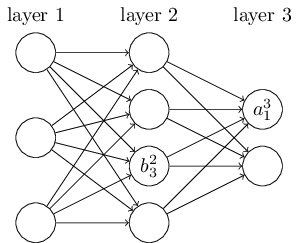
\includegraphics[height=2in, keepaspectratio=true]{exb.png}
\caption{Ký hiệu $bias$}
\end{figure}\\
Biễu diễn ma trận trọng số và vector $bias$:
\begin{itemize}
\item $w$ là ma trận của các giá trị trọng số.
\[ w =
\begin{bmatrix}
w_{11} & \ldots & w_{1k} \\
\vdots & \ddots & \vdots\\
w_{j1} & \ldots & w_{jk}
\end{bmatrix}
\]
\item $b$ là vector của các giá trị $bias$.
\[ b =
\begin{bmatrix}
b_1\\
\vdots\\
b_k
\end{bmatrix}
\]
\item $\sigma$ là hàm sigmoid.
\item $a_j=\sigma$ là hàm hoạt động có dạng sigmoid, $a$ là vector của các hàm 
hoạt động.
\[ a =
\begin{bmatrix}
a_1\\
\vdots\\
a_k
\end{bmatrix}
\]
\end{itemize}
Lúc này ta có biểu diễn toán học đầy đủ của hàm hoạt động:
\[
  a_j^\ell=\sigma(\sum_k w_{jk}^\ell a_k^{\ell-1} + b_j^\ell)=\sigma(z _j^\ell)
\]
\[
  z _j^\ell=\sum_k w_{jk}^\ell a_k^{\ell-1} + b_j^\ell
\]
Tổng quát phát biểu với dạng:\\
\[
  a^\ell=\sigma(w^\ell a^{\ell-1} + b^\ell)=\sigma(z^\ell)
\]
Để có thể tìm được giá trị của các biến $w$ và $b$, giải thuật lan truyền ngược 
thực hiện bằng cách xuất phát $w$ và $b$ từ các giá trị ngẫu nhiên, thực hiện 
các phép lặp để đưa $w$ và $b$ về giá trị đúng, mỗi lần lặp sẽ có một hàm chi 
phí (cost function) đo đạc độ lệch của giá trị tính toán và giá trị thực tế 
để giúp giải thuật tìm được giá trị hội tụ.\\\\
Biễu diễn hàm chi phí với $L$ lớp:
\[
  C=\frac{1}{2n}\sum_x\|y(x)-a^L(x)\|^2
\]
Ta có thể thấy, dạng hàm số trên tương đồng với định nghĩa độ lệch chuẩn trong 
xác suất thống kê nhưng có một số biến đổi khác biệt. Thay vì giá trị kỳ vọng 
và các giá trị xác suất, hàm chi phí sử dụng giá trị thực tế $y$ của tập dữ 
liệu và giá trị $y=a$ là giá trị $y$ tính toán được từ $x$ với $w$ và $b$. Vậy 
ta có thể hiểu được, hàm chi phí tính toán độ sai lệch của giá trị $a$ so với 
$y$ kỳ vọng thực tế. Do đó, hàm chi phí càng nhỏ thì biểu diễn giá trị của 
MNN sẽ càng gần với thực tế.\\\\
Để tìm được giá trị cực tiểu cho hàm chi phí ta sẽ thực hiện vòng lặp:
\[
  w_{jk}^\ell:=w_{jk}^\ell-\eta\frac{\partial}{\partial w_{jk}^\ell}C(w,b)
\]
\[
  b_j^\ell:=b_j^\ell-\eta\frac{\partial}{\partial b_j^\ell}C(w,b)
\]
Trong đó $\eta$ là tỉ lệ học (learning rate), việc hội tụ về giá trị cực tiểu 
với tốc độ và độ chính xác phụ thuộc vào tỉ lệ này. Thực hiện được hai vòng lặp 
trên, ta sử dụng giải thuật lan truyền ngược để tính toán 
$\frac{\partial}{\partial w_{jk}^\ell}C(w,b)$ và 
$\frac{\partial}{\partial b_j^\ell}C(w,b)$.\\\\
Tham số lỗi $\delta_j^\ell$ của neural thứ $j$ thuộc lớp $\ell$ là biểu diễn 
của:
\[
  \delta_j^\ell \equiv \frac{\partial C}{\partial z_j^\ell}
\]
Từ biểu diễn trên ta có:
\[
  \delta_j^L = \frac{\partial C}{\partial a_j^L} \sigma'(z_j^L)
\]
Mặc khác $\partial C/\partial a_j^L = (a_j^L-y_j)$, suy ra:
\[
  \delta^L=\nabla_aC\odot\sigma'(z^L)=(a^L-y)\odot\sigma'(z^L)
\]
Trong đó $\odot$ là tích Hadamard, ta gọi biểu thức trên là biểu thức (3.1).
Ngoài ra, ta có biểu diễn khác của $\delta_j^L$:
\begin{align*}
  \delta_j^L=\frac{\partial C}{\partial z_j^L}
  &=\sum_k\frac{\partial C}{\partial z_k^{\ell+1}}\frac{\partial z_k^{\ell+1}}{\partial z_j^\ell}\\
  &=\sum_k\frac{\partial z_k^{\ell+1}}{\partial z_j^\ell}\delta_k^{\ell+1}\\
  &=\sum_k\frac{\partial(\sum_j w_{kj}^{\ell+1}a_j^\ell+b_k^{\ell+1})}{\partial z_j^\ell}\delta_k^{\ell+1}\\
  &=\sum_k\frac{\partial(\sum_j w_{kj}^{\ell+1}\sigma(z_j^\ell)+b_k^{\ell+1})}{\partial z_j^\ell}\delta_k^{\ell+1}\\
  &=\sum_k w_{kj}^{\ell+1}\delta_k^{\ell+1}\sigma'(z_j^\ell)
\end{align*}
Gọi biểu thức trên là biểu thức (3.2). Với hướng tiếp cận tương tự ta có các 
biểu thức khác:
\begin{align*}
  \frac{\partial C}{\partial b_j^\ell}&=\frac{\partial C}{\partial z_j^\ell}\frac{\partial z_j^\ell}{\partial b_j^\ell}\\
  &=\delta_j^\ell\frac{\partial z_j^\ell}{\partial b_j^\ell}\\
  &=\delta_j^\ell\frac{\partial(\sum_k w_{jk}^\ell a_k^{\ell-1} + b_j^\ell)}{\partial b_j^\ell}\\
  &=\delta_j^\ell
\end{align*}
Ta có biểu thức trên là biểu thức (3.3).
\begin{align*}
  \frac{\partial C}{\partial w_{jk}^\ell}&=\frac{\partial C}{\partial z_j^\ell}\frac{\partial z_j^\ell}{\partial w_{jk}^\ell}\\
  &=\delta_j^\ell\frac{\partial(\sum_k w_{jk}^\ell a_k^{\ell-1} + b_j^\ell)}{\partial w_{jk}^\ell}\\
  &=\delta_j^\ell a_k^{\ell-1}
\end{align*}
Và biểu thức (3.4). Từ (3.1), (3.2), (3.3) và (3.4) ta có tổng kết sau:
\begin{align}
  \delta^L =& \: \nabla_aC\odot\sigma'(z^L) \\
  \delta^\ell =& \: ((w^{\ell+1})^T\delta^{\ell+1})\odot\sigma'(z^\ell) \\
  \frac{\partial C}{\partial b_j^\ell} =& \: \delta_j^\ell \\
  \frac{\partial C}{\partial w_{jk}^\ell} =& \: a_k^{\ell-1}\delta_j^\ell
\end{align}
Sử dụng các biểu thức này, giải thuật lan truyền ngược dùng để tính toán 
$\frac{\partial}{\partial w_{jk}^\ell}C(w,b)$ và 
$\frac{\partial}{\partial b_j^\ell}C(w,b)$ được mô tả các bước như sau:
\begin{enumerate}
\item Cho giá trị đầu vào $x$, tính toán giá trị $a^1$ tương ứng với $x$.
\item Với mỗi $\ell=2,3,..,L$, ta lần lượt tính được $z^\ell=w^\ell a^{\ell-1}+b^\ell$ 
và $a^\ell=\sigma(z^\ell)$.
\item Tính giá trị của vector $\delta^L=\nabla_aC\odot\sigma'(z^L)$.
\item Từ giá trị của $\delta^L$ ta có thể tính được giá trị của các tham số lỗi 
còn lại, với mỗi $\ell=L-1,L-2,...,2$ ta thực hiện $\delta^\ell=((w^{\ell+1})^T\delta^{\ell+1})\odot\sigma'(z^\ell)$.
\item Kết thúc quá trình tính toán với $\frac{\partial C}{\partial w_{jk}^\ell}=a_k^{\ell-1}\delta_j^\ell$ và 
$\frac{\partial C}{\partial b_j^\ell}=\delta_j^\ell$.
\end{enumerate}
\subsubsection{Thông số đánh giá}
Có ba tham số cơ bản dùng để xem xét và đánh giá kết quả giải thuật trong Học máy.
Ký hiệu: \textbf{True positive} là $TP$, \textbf{False positive} là $FP$, 
\textbf{True negative} là $TN$, \textbf{False negative} là $FN$.\\\\
Ta có:
\[
  Accuracy = \frac{TP+TN}{TP+FP+TN+FN}
\]
\[
  Precision = \frac{TP}{TP+FP}
\]
\[
  Recall = \frac{TP}{TP+FN}
\]
\begin{figure}[h!]
\centering
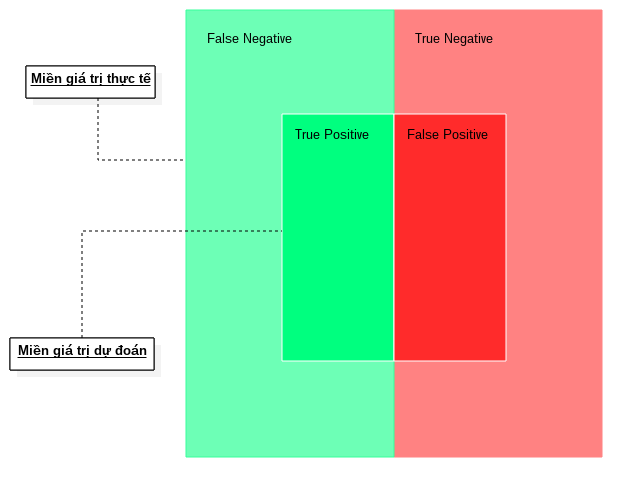
\includegraphics[height=2.5in, keepaspectratio=true]{precision_recall.png}
\caption{Thông số đánh giá}
\end{figure}
\section{Công trình liên quan}
Hai công trình được công bố công khai có đề tài tương đồng với đề tài của bài dự thi này đó là 
``Automated Bitcoin Trading via Machine Learning Algorithms'' \cite{AutomatedBitcoinTrading}
và ``Predicting the price of Bitcoin using Machine Learning'' \cite{PredictingThePriceOfBitcoin}.
Đây là hai công trình sử dụng trực tiếp Học máy trong bài toán dự đoán xu hướng 
giá trị BTC, mỗi công trình đều có một hướng tiếp cận riêng biệt và đồng thời 
cũng cho ra các kết quả khác nhau.\\\\
Trong bài báo \cite{AutomatedBitcoinTrading}, nhóm tác giả sử dụng một tập dữ 
liệu về giá trị BTC, tập dữ liệu này chứa khoảng 120.000 mẫu được thu thập thông 
qua API của Coinbase và OKCoin (đây là những loại ví điện tử được dùng để lưu 
trữ và trao đổi BTC, Coinbase xây dựng ở San Francisco và OKCoin xây dựng ở Bắc 
Kinh) - gọi đây là tập dữ liệu thứ nhất. Ngoài ra, nhóm tác giả còn thu thập 
thêm tập dữ liệu giá thường nhật kèm theo các thông tin về mạng Bitcoin, tập dữ 
liệu này bao gồm 26 đặc trưng nhưng chỉ được dùng 16 đặc trưng cho quá trình 
phân tích và chạy giải thuật - gọi đây là tập dữ liệu thứ hai.\\\\
Với tập dữ liệu thứ nhất, nhóm tác giả tiếp cận vấn đề bằng phương pháp chuỗi 
thời gian (Time Series) với 2 khoảng thang thời gian là 10 giây và 10 phút. Còn 
lại, tập dữ liệu thứ hai được sử dụng như một tập dữ liệu phân lớp đơn thuần.
Kết quả chi tiết của các giải thuật LR, SVM và RF:
\begin{table}[h]
\centering
\fontsize{8}{9}\selectfont
\begin{tabular}{ |c|c|c|c| }
\hline
Tham số đánh giá & 10 giây - LR & 10 phút - SVM & 10 phút - RF \\
\hline
Recall & 54.29\% & 52.40\% & 54.00\% \\
\hline
Specificity & 57.70\% & 57.60\% & 61.90\% \\
\hline
Precision & 57.40\% & 55.10\% & 58.10\% \\
\hline
Accuracy & 8.50\% & 53.90\% & 57.40\% \\
\hline
\end{tabular}
\caption{Bảng đánh giá với tập dữ liệu thứ nhất}
\end{table}\\
Lưu ý, nhóm tác giả ký hiệu giải thuật LR là Binomial GLM và tham số đánh giá 
Recall là Sensitivity.
\begin{table}[h]
\centering
\fontsize{8}{9}\selectfont
\begin{tabular}{ |c|c|c|c| }
\hline
Tham số đánh giá & LR & SVM & RF \\
\hline
Recall & 97.90\% & 3.48\% & 100\% \\
\hline
Specificity & 99.39\% & 55.14\% & 93.92\% \\
\hline
Precision & 97.90\% & 8.39\% & 77.62\% \\
\hline
Accuracy & 98.79\% & 27.16\% & 94.98\% \\
\hline
\end{tabular}
\caption{Bảng đánh giá với tập dữ liệu thứ hai}
\end{table}\\
Với công trình nghiên cứu \cite{PredictingThePriceOfBitcoin}, tác giả sử dụng 
một hướng tiếp cận khác hơn so với bài báo \cite{AutomatedBitcoinTrading}. Với 
tập dữ liệu giá BTC được thu thập thông qua CoinDesk từ ngày 19/8/2013 đến ngày 
19/07/2016, tác giả sử dụng các kiến thức về Học sâu (Deep Learning) như là một 
công cụ chính để phân tích và giải quyết bài toán. Ngoài ra, trong công trình 
này còn nhắc đến việc sử dụng mô hình ARIMA - một dạng mô hình phân tích chuỗi 
thời gian - như là một giải thuật dùng để so sánh với giải thuật chính. Giải 
thích quyết định này, tác giả đã đưa ra lý luận phân tích rằng, ARIMA mặc dù là 
một mô hình dữ đoán chuỗi thời gian phổ biến, tuy nhiên, mô hình này lại phụ 
thuộc vào giả định tập dữ liệu là tuyến tính về thời gian và điều này không phù 
hợp với tập dữ liệu đang được sử dụng - tập dữ liệu được sử dụng là phi tuyến 
tính.\\\\
Đi vào chi tiết, giải thuật học sâu được sử dụng đó là RNN một dạng của 
mạng neural (xem phần 3.3.3), RNN có khả năng sử dụng cả hai giải thuật lan 
truyền là lan truyền thuận và lan truyền ngược. Ngoài ra, tác giả còn sử dụng 
một biến thể khác của RNN, đó là LSTM, ở RNN các tham số mạng được tìm bằng 
giải thuật di truyền (Genetic Algorithm), khác với LSTM sử dụng giải thuật tối 
ưu Bayesian (Bayesian Optimisation) để tìm tham số mạng. Kết quả của quá trình 
chạy giải thuật:
\begin{table}[h]
\centering
\fontsize{8}{9}\selectfont
\begin{tabular}{ |c|c|c|c| }
\hline
Tham số đánh giá & LSTM & RNN & ARIMA \\
\hline
Recall & 37.00\% & 40.40\% & 14.7\% \\
\hline
Specificity & 61.30\% & 56.65\% & 100\% \\
\hline
Precision & 35.50\% & 39.08\% & 100\% \\
\hline
Accuracy & 52.78\% & 50.25\% & 50.05\% \\
\hline
\end{tabular}
\caption{Bảng đánh giá các giải thuật học sâu và ARIMA}
\end{table}\\
Ngoài hai công trình trên, chúng ta sẽ tiếp tục tham khảo các vấn đề liên quan 
khác như là dự đoán xu hướng giá trị vàng và dự đoán xu hướng giá trị cổ phiếu.
Mặc dù các công trình này không đi giải quyết vấn đề dự đoán giá trị BTC, nhưng 
với cách nhìn tổng quát, vấn đề chung vẫn là sử dụng Học máy để dự đoán giá trị 
các tài sản giao dịch. Vàng, cổ phiếu là hai tài sản giao dịch đặc trưng và lâu 
đời, vì thế các vấn đề về dự đoán của hai tài sản giao dịch này cũng đã được 
khai thác và phát triển từ lâu. Hai công trình cụ thể được tham khảo trong đề tài là: 
``Predicting Gold Prices'' \cite{PredictingGoldPrices} và 
``Machine Learning in Stock Price Trend Forecasting'' 
\cite{StockPriceTrendForecasting} \\\\ 
Bài báo \cite{PredictingGoldPrices} liên quan đến ứng dụng Học máy cho việc dự đoán 
giá vàng, tác giả đã chọn hướng tiếp cận học có giám sát và cụ thể là bài toán 
phân lớp. Tập dữ liệu mà tác giả sử dụng là tập dữ liệu giá vàng từ đầu năm 2007 
đến cuối năm 2013 với khoảng 1700 mẫu và được lấy từ trang web của USA Gold, 
đồng thời sử dụng hai giải thuật phân lớp là SVM và LR.
Trong đó, khi gặp phải vấn đề mất cân đối trong tập dữ liệu (nhãn $positive$ 
lớn hơn rất nhiều sao với nhãn $negative$) tác giả đã sử dụng giải thuật SVM 
với nhiều lần điều chỉnh mô hình như: sử dụng kernel RBF, sử dụng kernel tuyến 
tính với L1,... nhưng đều cho ra kết quả thấp (Accuracy nằm trong khoảng 50\% 
- 51\%). Với kết quả như vậy, tác giả đã quyết định sử dụng SVM như một giải 
thuật dùng để so sánh và đánh giá với giải thuật còn lại. Với một hướng tiếp 
cận khác, LR được sử dụng để giải quyết bài toán, kết quả được ghi nhận như 
bảng sau.
\begin{table}[h]
\centering
\fontsize{8}{9}\selectfont
\begin{tabular}{ |c|c| }
\hline
Precision & 69.90\% \\
\hline
Recall & 72.31\% \\
\hline
Accuracy & 69.30\% \\
\hline
\end{tabular}
\caption{Bảng đánh giá giải thuật LR}
\end{table}\\
Với kết quả trên, các tham số đánh giá cho kết quả trong khoảng gần bằng 70\% 
và tác giả xem đây là một kết quả có ý nghĩa.\\\\
Bài báo \cite{StockPriceTrendForecasting} liên quan đến ứng dụng Học máy cho việc 
dự đoán giá trị cổ phiếu (cụ thể là công ty 3M), nguồn dữ liệu được sử dụng là 
Bloomberg Data Terminal với khoảng 1400 mẫu. Nhóm tác giả đã sử dụng bốn 
giải thuật trong quá trình phân tích và giải quyết bài toán đó là: GDA, LR, SVM, 
QDA.\\\\
Ngoài ra, để có thể tìm ra một hướng giải quyết tối ưu, nhóm tác giả tiếp cận 
vấn đề dựa trên hai mô hình khác nhau. Thứ nhất, mô hình Ngày tiếp theo (Next-Day 
Model) với mục tiêu đi dự đoán xu hướng giá trị của cổ phiếu trong ngày tiếp 
theo. Và thứ hai, mô hình Dài hạn (Long-Term Model) với mục tiêu đi dự đoán xu 
hướng giá trị của $n$ ngày tiếp theo.\\\\
Kết quả đánh giá của 4 giải thuật cho mô hình Ngày tiếp theo:
\begin{table}[h]
\centering
\fontsize{8}{9}\selectfont
\begin{tabular}{ |c|c|c|c|c| }
\hline
Model & LR & GDA & QDA & SVM \\
\hline
Accuracy & 44.5\% & 46.4\% & 58.2\% & 55.2\% \\
\hline
\end{tabular}
\caption{Bảng đánh giá mô hình Ngày tiếp theo }
\end{table}\\
Đồ thị đánh giá của 4 giải thuật cho mô hình Dài hạn:
\begin{figure}[h!]
\centering
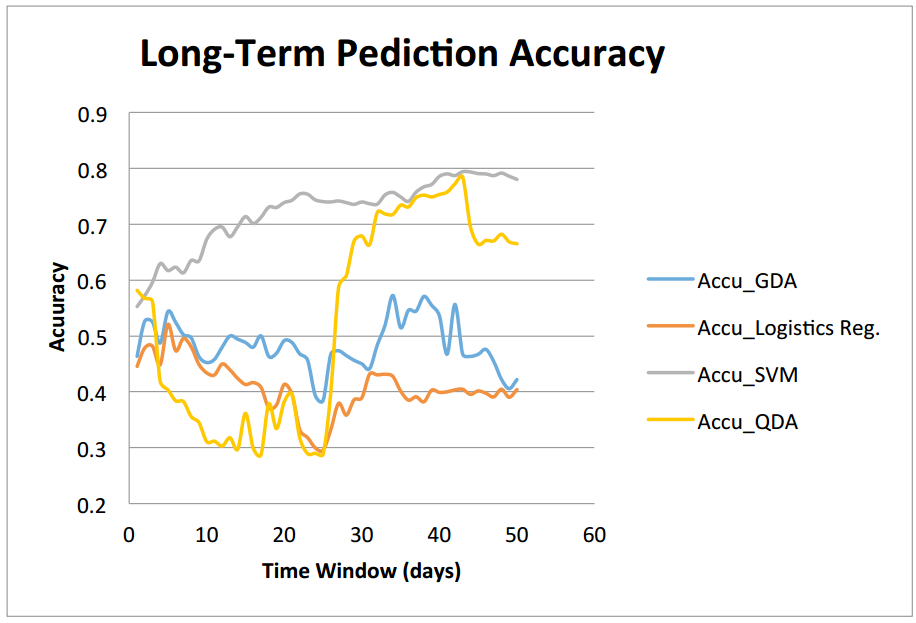
\includegraphics[height=2.15in, keepaspectratio=true]{longtermmodel.png}
\caption{Đồ thị đánh giá mô hình Dài hạn}
\end{figure}\\
Hai mô hình với hai kết quả, ta thấy ở mô hình Dài hạn hai giải thuật SVM và 
QDA cho kết quả Accuracy gần bằng 80\% với $n=44$ ngày, so sánh với mô hình 
Ngày tiếp theo Accuracy gần bằng 60\% ta có thể thấy mô hình dài hạn cho kết 
quả có ý nghĩa hơn. Nhưng một hạn chế rất lớn của công trình này, nhóm tác giả 
chỉ sử dụng một tham số đánh giá duy nhất là Accuracy mà bỏ qua Precision và 
Recall. Việc đánh giá chỉ dựa trên duy nhất một tham số sẽ không thể tổng quát 
được kết quả đầu ra, vì vậy mà dẫn đến nguy cơ không phát hiện các vấn đề về 
lệch dữ liệu hoặc overfitting.\\\\ 
Tổng quan qua các công trình trên và tham khảo một số công trình khác, nhận thấy 
đa số các hướng tiếp cận đều đi theo một phương pháp tổng quát chung và bao gồm 
các bước cơ bản như:
\begin{enumerate}
\item Xây dựng không gian vector đặc trưng phù hợp với tính chất bài toán
\item Lựa chọn mô hình phân tích
\item Sử dụng các giải thuật phân lớp điển hình trong Học máy như là 
SVM, LR ...
\item Đánh giá giải thuật bằng các tham số Accuracy, Recall, Precision.
\end{enumerate}
\section{Thu thập dữ liệu và lựa chọn giải thuật}
\subsection{Thu thập dữ liệu}
\subsubsection{Nguồn dữ liệu}
Poloniex là một sàn giao dịch tiền mã hóa trực tuyến và có trụ sở tại Mỹ. Được 
thành lập vào tháng 1 năm 2014, khi đi vào hoạt động, Poloniex định hướng cung 
cấp một môi trường thương mại an toàn, đồng thời còn cung cấp các dữ liệu về 
thị trường như biểu đồ, bảng xếp hạng và các công cụ phân tích dữ liệu để hỗ 
trợ khách hàng. Ngoài ra, Poloniex còn cung cấp một số lượng dữ liệu liên quan 
đến các thống kê mua/bán của sàn giao dịch, các dữ liệu này được cung cấp thông qua API.\\\\ 
Nguồn dữ liệu được lấy thông qua API dữ liệu biểu đồ thị trường của sàn giao 
dịch Poloniex. Cụ thể API:
\begin{lstlisting}
https://poloniex.com/public?command=returnChartData&currencyPair=BTC_XMR&start=1405699200&end=9999999999&period=14400
\end{lstlisting}
Tập dữ liệu về các phiên giao dịch Bitcoin được thu thập từ ngày 20/2/2015 đến 
ngày 29/10/2016 và có tổng cộng 29634 mẫu (mỗi mẫu là đại diện của một phiên 
giao dịch).
Dữ liệu trả về là một mảng các phần tử JSON có dạng như sau:
\begin{lstlisting}
[
    {"date":1424372400,"high":225,"low":225,"open":225,"close":225,"volume":0.999999,"quoteVolume":0.00444444,"weightedAverage":225},
    {"date":1424374200,"high":225,"low":225,"open":225,"close":225,"volume":0,"quoteVolume":0,"weightedAverage":225},
    ...,
    {"date":1482575400,"high":900.79862142,"low":894.98864451,"open":900.79862142,"close":895.56277339,"volume":2427.10998126,"quoteVolume":2.70065724,"weightedAverage":898.71085649}
]
\end{lstlisting}
Sau khi thu thập, dữ liệu được tiền xử lý để loại bỏ các thông tin không được 
sử dụng trong quá trình phân tích và xây dựng giải thuật. Giá trị có khóa là 
$close$ là dữ liệu sẽ được sử dụng, các giá trị như: $date$, $high$, $low$, 
$open$, $volume$, $quoteVolume$, $weightedAverage$ sẽ được lược bỏ.
\subsubsection{Xây dựng dữ liệu luyện tập}
Gọi $S$ là đại diện cho một phiên giao dịch, các đặc trưng được xây dựng như 
sau:
\begin{itemize}
    \item 10 feature RDP: $\{ \: loop\{ RDP_1(S_{i+j})\}_i \: \}_j$ Với 
    $i \in [0:9], \: j \in [0:29634]$
    \item 1 feature SO. Với $ j \in [0:29625] $:\\
    \[
        \{ \%K_j = \frac{P(j+9)-L_{10}}{H_{10}-L_{10}} \}_j
    \]
    \item 1 feature ROC. Với $ j \in [0:29625] $:\\ 
    \[
        \{ ROC_{10}(j)= \frac{P(j+9) - P(j)}{P(j)} \}_j
    \]
\end{itemize}
Ở đây, chúng ta chọn mỗi vector đặc trưng được hình thành bởi 10 phiên giao 
dịch. Các giá trị SO và ROC đều được tính trong thời gian là 10 phiên giao dịch.
Sau khi đã có tập luyện tập (tập hợp các vector đặc trưng), ta cần nhãn - label 
để phân lớp tập luyện tập. Nhãn được định nghĩa như sau, nếu giá BTC ở phiên 
thứ 11 lớn hơn phiên thứ 10 thì nhãn sẽ là 1, ngược lại sẽ là 0 (Phiên 11 chính 
là phiên thứ 1 của nhóm 10 phiên liền sau nhóm 10 phiên hiện đang xét).\\
\[
    label_i = \bigg \{ _{0 \quad if \: P_i(10) \: \leq \: P_{i+1}(1)} ^{1 \quad if \: P_i(10) \: > \: P_{i+1}(1)}
\]
Kết quả dữ liệu luyện tập:
\begin{lstlisting}
0 0.06666666666666667 0.016666666666666666 0 0 0 0 0 0 0 0.08444444444444445 1 0
0.06666666666666667 0.016666666666666666 0 0 0 0 0 0 0 0 0.016666666666666666 1 0
...
0.002400968290280231 3.9565217470358025e-9 0.003910087158215986 -0.00045140752064857115 -0.0013329209110243738 0.0008262923440509297 0.018429551716218056 0.003236901952232515 -0.004644611078085971 -0.0016267310238298762 0.018318840535169866 0.7405268424216611 0
\end{lstlisting}
Mỗi hàng đại diện cho một vector đặc trưng và nhãn, chi tiết ở một vector đặc 
trưng 10 giá trị đầu sẽ là 10 đặc trưng $RDP$, 1 giá trị tiếp theo là đặc trưng 
$ROC$, 1 giá trị tiếp theo là đặc trưng $SO$ và 1 giá trị cuối cùng là nhãn.

\subsection{Lựa chọn giải thuật}
Bên cạnh chạy giải thuật MNN, chúng ta sẽ chạy các giải thuật khác nhằm so sánh 
và đánh giá giải thuật chính. Các giải thuật được chọn để so sánh với giải thuật 
chính: SVM (Support Vetor Machines), KNN (K-Nearest Neighbors), LR (Logistic Regression).\\\\
Để đánh giá mức độ ý nghĩa của từng giải thuật, chúng ta sẽ sử dụng 3 tham số 
đánh giá là Accuracy, Recall, Precision. Tập dữ liệu sẽ được chia ra thành hai phần:
\begin{itemize}
\item Tập huấn luyện: chiếm 7/10 tổng số dữ liệu, dùng để chạy trong quá trình 
học của giải thuật.
\item Tập đánh giá: chiếm 3/10 tổng số dữ liệu, dùng để chạy trong quá trình 
đánh giá giải thuật.
\end{itemize}
Mô hình đánh giá giải thuật được mô tả bằng cách, dùng tập huấn luyện để tạo 
ra mô hình học máy của các giải thuật, sau đó sử dụng tập đánh giá để làm đầu 
vào cho từng mô hình, kết quả dự đoán sẽ được so sánh với kết quả thực tế của 
từng vector đặc trưng đầu vào. Cụ thể, kết quả của 4 giải thuật được ghi nhận 
như sau:
\begin{table}[h]
\centering
\fontsize{8}{9}\selectfont
\begin{tabular}{ |c|c|c|c|c| }
\hline
 & KNN & LR & SVM & MNN \\
\hline
Accuracy & 62.93\% & 66.24\% & 66.40\% & 69.86\% \\
\hline
Precision & 44.69\% & 18.18\% & 0\% & 60.50\% \\
\hline
Recall & 43.62\% & 0.15\% & 0\% & 29.55\% \\
\hline
\end{tabular}
\caption{Bảng đánh giá}
\end{table}\\
Trước tiên theo bảng đánh giá, ta có các giải thuật LR và SVM cho kết quả Accuracy
là gần khoảng 66\%, nhưng khi nhìn vào chi tiết các giá trị Precision và Recall 
ta nhận thấy kết quả điều cho ra rất thấp. Kết quả này cho thấy giải thuật LR 
và SVM đều có số lần True Positive là xấp xỉ bằng 0, đồng nghĩa với việc các 
giải thuật này hầu như chỉ dự đoán kết quả là nhãn $Down$ cho tất cả trường hợp. 
Điều này hoàn toàn không có ý nghĩa trong dự đoán đầu tư.\\\\
Xét đến KNN và MNN, đối với KNN ta có thể thấy giải thuật có xu hướng cân bằng 
các giá trị Accuracy, Precision và Recall. Nhưng đối với MNN, giải thuật có xu 
hướng tối ưu hóa bộ thiêu chuẩn Accuracy và Precision. Vậy câu hỏi đặt ra ở đây 
là kết quả nào có giá trị đầu tư hơn?\\\\
Chú ý đến Recall, dựa theo định nghĩa thì Recall có thể hiểu nếu trong thực tế 
có 10 phiên là $Up$ thì KNN sẽ dự đoán đúng khoảng 4 lần và MNN sẽ dự đoán đúng 
khoảng 3 lần. Điều này có nghĩa là KNN sẽ chiếm ưu thế so MNN khi sử dụng tiêu 
chuẩn là Recall.\\\\
Xét đến Precision, ta có thể hiểu Precision như sau, với 10 lần dự đoán sẽ có 
phiên $Up$ thì KNN sẽ đúng khoảng 4 lần và MNN sẽ dự đoán đúng 6 lần. Giả sử, 
mức độ tin tưởng của chúng ta vào hệ thống là 100\%, cứ mỗi lần hệ thống dự 
đoán có phiên $Up$ thì ta sẽ quyết định đầu tư. Điều đó đồng nghĩa, nếu theo 
KNN sẽ có 6 lần ta chịu lỗ vì hệ thống dự đoán sai và với MNN thì ta sẽ có 4 
lần ta chịu lỗ.\\\\
Quay lại với Recall, giá trị này không đo đạt được việc chúng ta sẽ lợi nhuận 
hoặc thua lỗ ra sao mà thực ra là giá trị đo đạt khả năng tận dụng cơ hội của 
hệ thống.\\\\
Tới lúc này, ta có thể kết luận, bộ tiêu chuẩn chiếm ưu thế cao hơn sẽ là Accuracy 
và Precision. Điều đó cũng có nghĩa là giải thuật MNN cho kết quả ý nghĩa hơn so 
với KNN và sẽ được lựa chọn để giải quyết bài toán dự đoán xu hướng giá trị BTC.
\section{Xây dựng hệ thống}
Hệ thống được xây dựng với mục tiêu là một ứng dụng nền web, cung cấp công cụ hỗ 
trợ cho việc dự đoán xu hướng giá trị BTC.
\subsection{Tổng quan hệ thống}
Hệ thống được xem xét và được thiết kế với 3 khối máy chủ , mỗi khối máy chủ đại 
diện cho một khối chức năng riêng biệt. Cấu trúc hệ thống như vậy nhằm dự trù và đảm bảo 
cho các hoạt động về quản lý hệ thống như phân phối tải, bảo trì và mở rộng sau 
này được thực hiện dễ dàng và tiết kiệm thời gian. Chi tiết các hệ thống máy chủ:
\begin{itemize}
\item Hệ thống máy chủ học máy - Machine Learning server
\item Hệ thống máy chủ backend - Backend server
\item Hệ thống máy chủ UI frontend - UI Frontend server
\end{itemize}
Các khối hệ thống giao tiếp với nhau bằng API và Socket - đối với các chức năng
chạy thời gian thực.\\
\begin{figure}[h!]
\centering
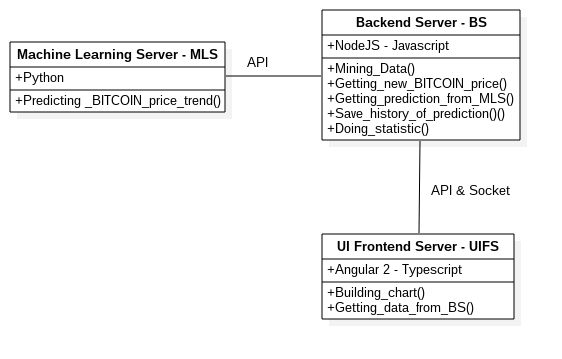
\includegraphics[height=2in, keepaspectratio=true]{system.png}
\caption{Cấu trúc quan hệ và chức năng hệ thống}
\end{figure}
\subsection{Hệ thống máy chủ học máy}
Đây là hệ thống cốt lõi của của sản phẩm, nó đảm nhiệm khối chức năng chính 
liên quan đến các tác vụ học máy, cụ thể, dựa vào các tham số được truyền vào 
để thực hiện quá trình chạy giải thuật dự đoán từ đó đưa ra giá trị nhãn dự 
đoán tương ứng cho bộ tham số đó.\\\\
Hệ thống máy chủ học máy được chia thành hai phần:
\begin{enumerate}
\item Prediction: bao gồm các chức năng đọc mô hình MNN đã xây dựng, chạy mô 
hình với tham số truyền vào và lấy các kết quả đầu ra.Kết quả đầu ra có giá 
trị nhãn $Up-Down$ và xác suất dự đoán.
\item Django: bao gồm các chức năng để trở thành một máy chủ giao tiếp thông 
qua API, các chức năng có thể ví dụ như tiếp nhận các yêu cầu thông qua API, 
phản hồi các yêu cầu dưới dạng các kết quả JSON...
\end{enumerate}
\subsection{ Hệ thống máy chủ backend}
Vì bản thân hệ thống máy chủ học máy không có các khối chức năng liên quan đến 
việc lấy dữ liệu giá BTC cũng như khai phá dữ liệu, nên hệ thống máy chủ backend 
được xây dựng để thực hiện các chức năng này. Đồng thời, máy chủ backend còn là 
cầu nối giữa trải nghiệm người dùng (hệ thống máy chủ UI frontend) và hệ thống 
máy chủ học máy.\\\\
Để thực hiện được công việc trên, hệ thống bao gồm được xây dựng các chức năng:
\begin{enumerate}
\item Cập nhật giá BTC: thông qua các public API được sàn giao dịch Poloniex 
cung cấp, các hàm lấy giá được chạy liên tục để cập nhật giá BTC mới nhất nhằm 
phục vụ cho quá trình dự đoán (trung bình 20 giây).
\item Khai phá dữ liệu: dữ liệu được các hàm cập nhật giá BTC lấy được vẫn 
còn ở dạng thô, chưa qua xử lý. Khai phá dữ liệu là biến đổi các dữ liệu này 
về các bộ tham số có ý nghĩa với Học máy, các giá trị này mới đích thực 
dùng để làm đầu vào dự đoán xu hướng giá trị BTC.
\item Giao tiếp với hệ thống máy chủ học máy: truyền tham số đi và nhận 
kết quả trả về từ hệ thống máy chủ học máy thông qua API.
\item Lưu trữ và thống kê dữ liệu: thực hiện việc lưu trữ dữ liệu, từ đó tạo 
nên một hệ thống các dữ liệu phục vụ cho việc phân tích, thống kê để cung cấp 
cho người dùng đầu cuối. Đó là các thông tin hết sức quý giá phục vụ cho các 
nhà đầu tư.
\item Giao tiếp với hệ thống máy chủ UI frontend: đưa ra những API chức năng 
nhằm phục vụ cho máy chủ UI frontend. Ví dụ như: yêu cầu dữ liệu dự đoán, yêu 
cầu thống kê đúng/sai, yêu cầu dữ liệu giá cho biểu đồ...
\end{enumerate}
\subsection{Hệ thống máy chủ UI frontend}
Hệ thống máy chủ UI frontend là một giao diện người dùng, nó cho phép người 
dùng có thể tiếp cận với các chức năng của toàn bộ hệ thống một cách dễ dàng. 
Hệ thống bao gồm nhiều biểu đồ, cũng như tham số cung cấp các thông tin có ý 
nghĩa đầu tư - dự đoán xu hướng giá trị Bitcoin - đồng thời với đó, là các 
thông tin về độ tin cậy của hệ thống, các thống kê về lịch sử dự đoán...\\\\
Một số hình ảnh về hệ thống thực tế.\\
\begin{figure}[h!]
\centering
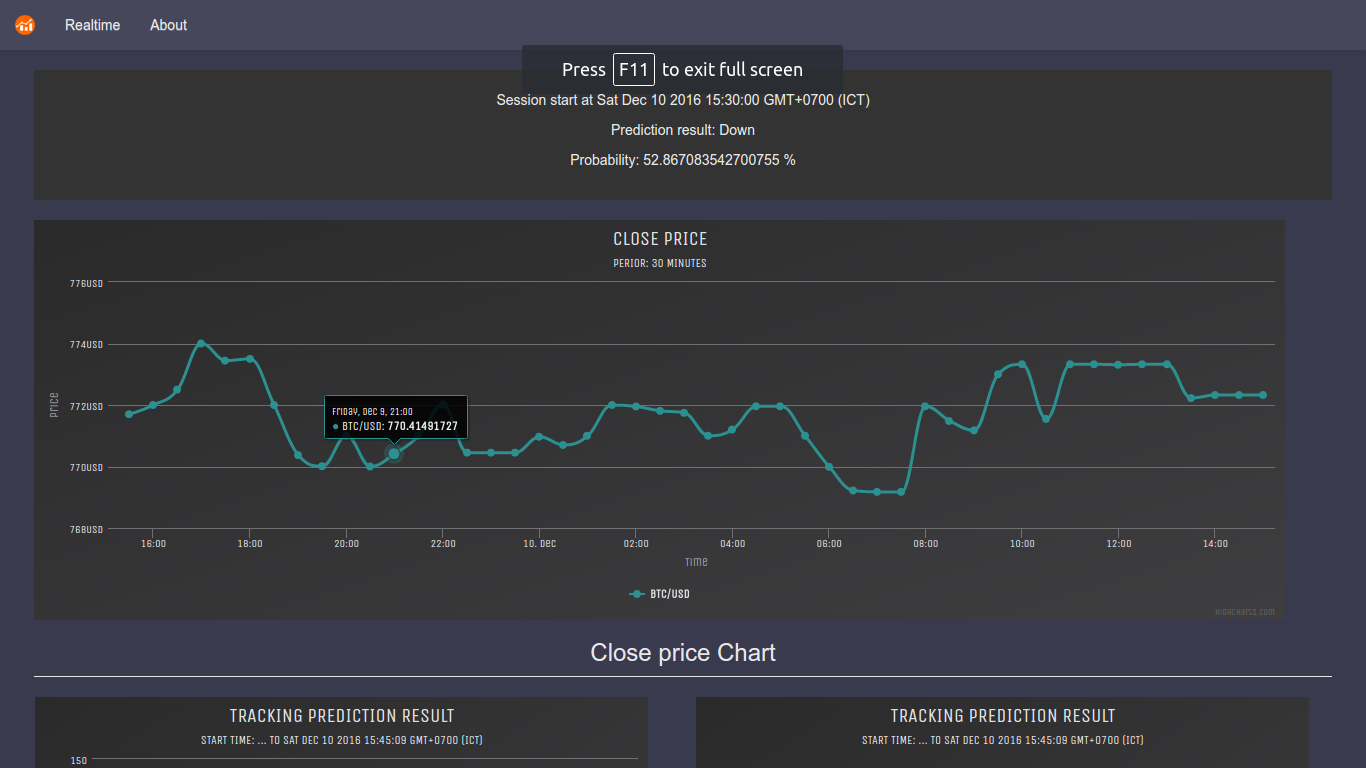
\includegraphics[height=2in, keepaspectratio=true]{2.png}
\caption{Giao diện 2 máy chủ UI frontend}
\end{figure}\\
\begin{figure}[h!]
\centering
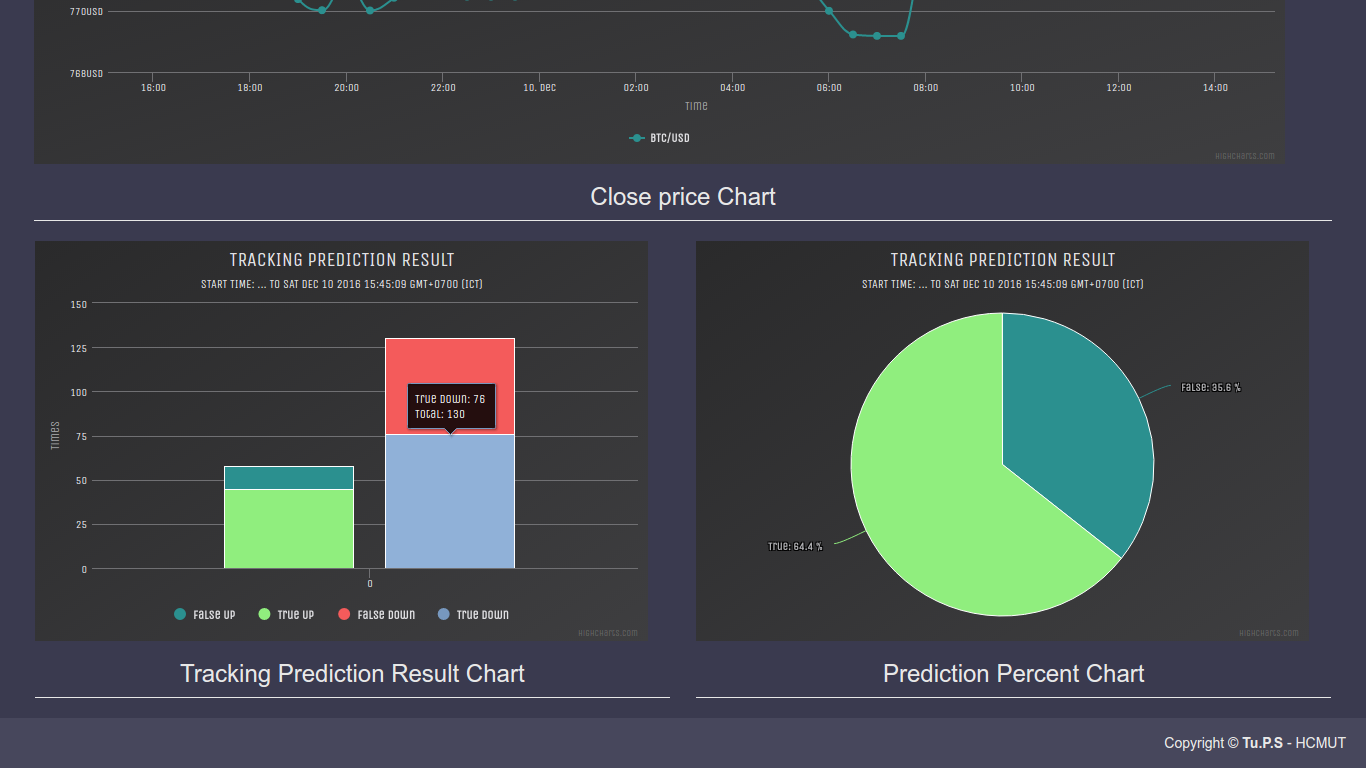
\includegraphics[height=2in, keepaspectratio=true]{3.png}
\caption{Giao diện 3 máy chủ UI frontend}
\end{figure}\\\\
\section{Kết luận và hướng phát triển}
\subsection{Kết luận}
Kết thúc đề tài, sản phẩm cuối cùng được hoàn thiện là một công cụ nền Web hỗ 
trợ, cung cấp các thông tin có giá trị tham khảo để đầu tư Bitcoin. Dựa trên 
các con số lý thuyết, khả năng dự đoán chính xác là rất khả quan và đặc biệt, 
giải thuật được tối ưu cho phù hợp với góc nhìn của một người đầu tư.\\\\
Với không nhiều sai lệch khi so sánh bên cạnh các con số lý thuyết, khi hệ thống được cho chạy 
thực tế trong vòng 4 ngày liên tiếp (Cụ thể từ 22:30:00 13/11/2016 đến 
20:30:00 17/11/2016) đã cho ra kết quả:\\
\begin{table}[h]
\centering
\fontsize{8}{9}\selectfont
\begin{tabular}{ |c|c|c| }
\hline
Accuracy & Precision & Recall \\
\hline
64.4\% & 77.6\% & 45.5\% \\
\hline
\end{tabular}
\caption{Bảng đánh giá hệ thống thực tế }
\end{table}\\
Các tham số đánh giá chạy thực tế như vậy, có thể thấy với một lần đầu tư 
ta có tới hơn 70\% là có lợi nhuận. Tuy vậy, bất kỳ một hệ thống cũng vẫn 
sẽ có những điểm thiếu sót.\\\\
Vì giới hạn của thời gian thực hiện đề tài, phạm vi của đề tài cũng được thu 
hẹp để phù hợp nên vì thế đã bỏ qua một số yếu tố thị trường ảnh hưởng khá lớn 
đối với hướng giải quyết. Trong lúc này, bản thân có thể nhận ra hai vấn đề:
\begin{itemize}
\item Phí giao dịch: ở tất cả các sàn giao dịch, đều có một khoảng phí trung gian 
từ 0.1\% đến 0.3\% và phí này được trừ trực tiếp vào các giao dịch. Hướng tiếp 
cận của đề tài bỏ qua hoàn toàn yếu tố này và có thể hiểu là phí bằng 0\%
\item Biên độ lợi nhuận và thua lỗ: chúng ta cũng đã bỏ qua yếu tố này, mặc dù 
dựa theo đánh giá thì số lần đầu tư lợi nhuận sẽ nhiều hơn thua lỗ. Nhưng, chúng 
ta không thể kết luận việc đầu tư sẽ chắc chắn đem về lợi nhuận. Hãy nói đến một 
trường hợp xấu, biên độ lợi nhuận chỉ có \$1 cho mỗi lần nhưng biên độ thua lô 
lại là \$100, tại đây chúng ta có thể thấy là việc đầu tư không hề có lợi.
\end{itemize}
Việc nhìn nhận được các vấn đề trên không hẳn là điều tồi tệ, mà ngược lại giúp 
chúng ta có thể hiểu rõ bài toán và đưa ra những hướng phát triển tiếp theo.
\subsection{Hướng phát triển}
Với các vấn đề còn tồn tại được nêu ra bên trên (Mục 5.1), giai đoạn tiếp theo 
của đề tài là đi giải quyết vẫn đề tài như hiện giờ nhưng thêm vào đó là yếu 
tố phí giao dịch. Tuy là một yếu tố nhỏ nhưng nó dẫn đến việc thay đổi hoàn toàn 
bộ dữ liệu ban đầu, điều này đồng nghĩa toàn bộ hệ thống hiện giờ sẽ không 
tương thích. Vì thế, cần thực hiện lại quá trình xây dựng giải thuật từ đầu.\\\\
Mặc khác, việc chỉ học duy nhất từ tập dữ liệu về giá BTC là không đủ để 
đưa ra một dự đoán chính xác cao. Ngày nay, mạng xã hội đang phát triển như vũ 
bão, đây là một kênh thông tin cực kỳ quý giá, chính vì vậy mà hệ thống ở giai 
đoạn phát triển tiếp theo sự tận dụng tài nguyên này.\\\\
Phát triển hệ thống xử lý ngôn ngữ tự nhiên, xây dựng hệ thống lắng nghe các 
thông tin tài chính, chính trị có ảnh hưởng tới giá trị BTC, phân tích, 
đánh giá và cho cân bằng với hệ thống học từ dữ liệu giá BTC để cho ra một 
dự đoán tổng quát và chính xác hơn.\\\\
Đồng thời, hệ thống có thể mở rộng ra cho nhiều loại tiền mã hóa khác như: 
Ethereum, Zcash, Monero...




% if have a single appendix:
%\appendix[Proof of the Zonklar Equations]
% or
%\appendix  % for no appendix heading
% do not use \section anymore after \appendix, only \section*
% is possibly needed

% use appendices with more than one appendix
% then use \section to start each appendix
% you must declare a \section before using any
% \subsection or using \label (\appendices by itself
% starts a section numbered zero.)
%


% \appendices
% \section{Proof of the First Zonklar Equation}
% \blindtext

% use section* for acknowledgement
% \section*{Acknowledgment}


% The authors would like to thank...


% Can use something like this to put references on a page
% by themselves when using endfloat and the captionsoff option.
\ifCLASSOPTIONcaptionsoff
  \newpage
\fi



% trigger a \newpage just before the given reference
% number - used to balance the columns on the last page
% adjust value as needed - may need to be readjusted if
% the document is modified later
%\IEEEtriggeratref{8}
% The "triggered" command can be changed if desired:
%\IEEEtriggercmd{\enlargethispage{-5in}}

% references section

% can use a bibliography generated by BibTeX as a .bbl file
% BibTeX documentation can be easily obtained at:
% http://www.ctan.org/tex-archive/biblio/bibtex/contrib/doc/
% The IEEEtran BibTeX style support page is at:
% http://www.michaelshell.org/tex/ieeetran/bibtex/
%\bibliographystyle{IEEEtran}
% argument is your BibTeX string definitions and bibliography database(s)
%\bibliography{IEEEabrv,../bib/paper}
%
% <OR> manually copy in the resultant .bbl file
% set second argument of \begin to the number of references
% (used to reserve space for the reference number labels box)
\begin{thebibliography}{1}

\bibitem{Bitcoin1}
Hough, Jack (3/6/2011). ``The Currency That's Up 200,000\%''. SmartMoney (Dow Jones \& Company). Truy cập 24/12/2016.
\bibitem{Bitcoin2}
Wallace, Benjamin (23/11/2011). ``The Rise and Fall of Bitcoin''. Wired. Truy cập 24/12/2016.
\bibitem{Bitcoin3}
Marc Kenigsberg (26/10/2013). ``BTC vs mBTC vs uBTC''. Bitcoinchaser. Truy cập 24/12/2016.
\bibitem{LawBitcoin}
Đồng Bitcoin (04/2016). ``Liên minh châu âu đã công nhận Bitcoin''. DongBitcoin. Truy cập 25/12/2016.
\bibitem{BitcoinPaper}
Satoshi Nakamoto (2008). Bitcoin: A Peer-to-Peer Electronic Cash System.
\bibitem{AutomatedBitcoinTrading}
I. Madan, S. Saluja và A. Zhao (2014). Automated Bitcoin Trading via Machine Learning Algorithms.
\bibitem{PredictingThePriceOfBitcoin}
Sean McNally (22/08/2016). \emph{Predicting the price of Bitcoin using Machine Learning}. MSc Reseach Project, National College of Ireland.
\bibitem{PredictingGoldPrices}
Megan Potoski (2013). Predicting Gold Prices. 
\bibitem{StockPriceTrendForecasting}
Yuqing Dai \& Yuning Zhang (2013). Machine Learning in Stock Price Trend Forecasting.
\bibitem{NeuralNetworksandDeepLearning}
Michael Nielsen (1/2016). \emph{Neural Networks and Deep Learning}. [Online]. Nguồn: http://neuralnetworksanddeeplearning.com/ 

\end{thebibliography}

% biography section
% 
% If you have an EPS/PDF photo (graphicx package needed) extra braces are
% needed around the contents of the optional argument to biography to prevent
% the LaTeX parser from getting confused when it sees the complicated
% \includegraphics command within an optional argument. (You could create
% your own custom macro containing the \includegraphics command to make things
% simpler here.)
%\begin{biography}[{\includegraphics[width=1in,height=1.25in,clip,keepaspectratio]{mshell}}]{Michael Shell}
% or if you just want to reserve a space for a photo:

\begin{IEEEbiography}[{\includegraphics[width=1in,height=1.25in,clip,keepaspectratio]{picture}}]{John Doe}
\blindtext
\end{IEEEbiography}

% You can push biographies down or up by placing
% a \vfill before or after them. The appropriate
% use of \vfill depends on what kind of text is
% on the last page and whether or not the columns
% are being equalized.

%\vfill

% Can be used to pull up biographies so that the bottom of the last one
% is flush with the other column.
%\enlargethispage{-5in}




% that's all folks
\end{document}


